\section{Experiment}
To verify the reliability of the water balance model for high-power fuel cell systems, it is necessary to record the water-containing state of the high-power fuel cell system when it reaches water balance under different operating conditions. Therefore, the experimental conditions should meet the following three points:(1) : The selected operating parameters should be within the normal operating range of the fuel cell system to avoid other faults in the fuel cell system other than water content faults (such as insufficient supply of reaction gas, air compressor surge, proportional valve failure, etc.), (2)In order to study the phenomena when the fuel cell system has a water content fault, the designed experiment needs to reflect more obvious phenomena under dry and flooded conditions, (3) The steady-state operation time should be long enough to ensure that the water content inside the fuel cell is in dynamic balance during this period, avoiding the impact of dynamic characteristics on the experimental results.
\subsection{Experiment Design}
The literature indicates that the factors that have the greatest impact on the water content inside the fuel cell are the air metering ratio, working temperature, and load current \cite{legrosFirstResultsPEMFC2011}. Since the temperature inside the stack cannot be measured during operation, the inlet temperature of the coolant is used as the working temperature in this paper, and the working temperature in the following text refers to the inlet temperature of the coolant. According to the operating conditions recommended by the system side, a three-factor five-level water content experiment was designed. The parameters of the experiment are shown in \ref{tab:WaterStateExperimentalParameterTable}.
\begin{table}
    \centering
    \begin{center}
    \caption{Water state experimental parameter table}
    \label{tab:WaterStateExperimentalParameterTable}
    \begin{tabular}{l|c|r}
        \hline
        \textbf{Load current/A/currency density/A·cm-2} & \textbf{Working temperature/℃} & \textbf{Air metering ratio}\\
        \hline
        120/0.4 & 55,60,65,70,73 & 2,2.2,2.4,2.6,2.8\\
        210/0.7 & 55,60,65,70,73 & 1.8,2,2.2,2.4 \\
        300/1.0 & 63,65,68,70,73 & 1.8,2,2.2,2.4 \\
        \hline
        
    \end{tabular}
\end{center}
\end{table}

Literatures\cite{wuDiagnosticToolsPEM2008} indicates that the time required for the fuel cell system to reach water balance is generally a few seconds to ten minutes. Therefore, each test point ran for 20 minutes, and it was assumed that the fuel cell was in the process of establishing water balance within the first 15 minutes, and no data was recorded for this process, and the data obtained in the last 5 minutes was recorded. During the test, if a single cell voltage is too low or other faults cause the fuel cell system to shut down, the data of this operating point will be removed.


\subsection{Test platform introduction}
The high-power fuel cell system used in this article is shown in Fig 2, manufactured by AT\&M Environmental Engineering Technology Co. The rated net output power of the fuel cell system is 100kW, the stack is composed of 410 single cells. High-pressure dry hydrogen gas enters the anode of the reaction stack after being depressurized by the solenoid valve and proportional valve. The liquid water in the residual hydrogen is separated by the gas-water separation device and intermittently discharged through the drain valve.
\begin{figure}[h]
    \centering
    \label{fig:PowerSystemDiagram}
    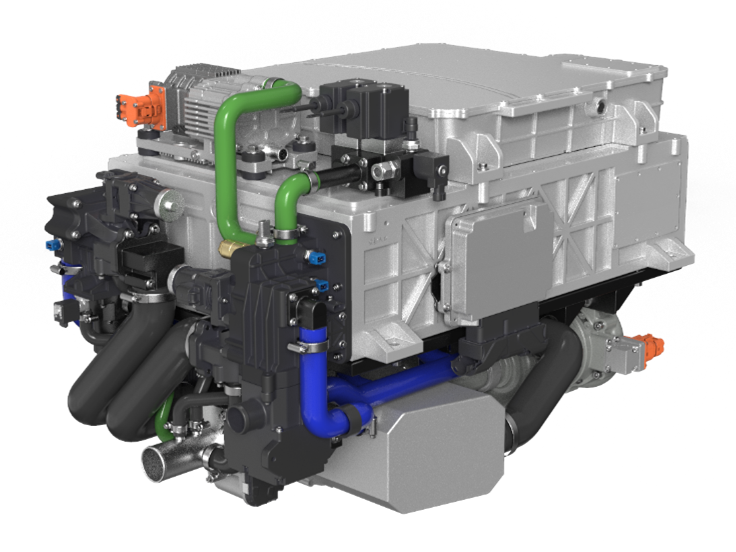
\includegraphics[scale=0.4]{Research_pictures/picture2.png}
    \caption[short]{power system diagram}
\end{figure}

For the above fuel cell system, the water balance model can be represented as

